\documentclass[12pt]{article}
\usepackage[utf8]{inputenc}
\usepackage[T2A, T1]{fontenc}
\usepackage{expex}
\lingset{aboveglftskip=-.2ex,interpartskip=\baselineskip,everyglb=\normalsize}
\usepackage[russian,english]{babel}
\usepackage{tipa}
\usepackage{coling2018}
\usepackage{times}
\usepackage{url}
\usepackage{latexsym}
\usepackage{booktabs}
\usepackage{adjustbox}
\usepackage{graphicx}
\usepackage{verbatim}
\usepackage{longtable}
\usepackage{textcomp}
\usepackage[letterpaper,margin=1in]{geometry}
\usepackage{setspace}
\doublespacing
\pagenumbering{arabic}

\usepackage{todonotes}
\newcommand{\note}[4][]{\todo[author=#2,color=#3,size=\scriptsize,fancyline,caption={},#1]{#4}}
\newcommand{\mans}[2][]{\note[#1]{MH}{blue!40}{#2}{}}   
\newcommand{\Mans}[2][]{\mans[inline,#1]{#2}\noindent}

\pagestyle{plain}

\title{Computational Morphology in Low Resource Settings}
\author{\\Synthesis Paper \\ Sarah R. Moeller}
\date{}

\begin{document}

\maketitle

\section{Introduction}

This paper examines if it possible to apply computational methods to the analysis of morphology in low resource contexts, particularly language documentation and description (LDD) data.\footnote{``Language documentation and description'' (LDD) data refers to resources that results from linguistic fieldwork and basic linguistic analysis. ``low resource languages'' (LRL), according to LORELEI (a US-government funded project for building language technology in low resource languages), refers to languages for which no automated human language technology exists, typically because of a lack of available linguistic resources. Other terms are sometimes used: ``under-described languages'' could be described as having minimal published descriptive linguistic resources, what \newcite{duong_natural_2017} calls ``very scarce-resource language;'' ``under-documented languages'', or Duong's ``extremely scarce-resource languages,'' lack sufficient raw or annotated data to write a full descriptive grammar; ``endangered languages'' are predicted to have no native speakers within a generation or two and most are under-documented and/or under-described. These distinctions are rarely crucial in this paper and can be understood almost interchangeably.} It attempts to identify what models or techniques are missing from linguistic fieldwork. In this paper, a question that represents ``uncharted territory for NLP [natural language processing]'' is directed specifically to morphology: ``What [computational] methods do we have that can detect structure in small, noisy data sets, while being directly applicable to a wide variety of languages?'' \cite[page 472]{bird_natural_2009}. 

Morphology comprises word-building properties in human languages and their accompanying (morpho-)syntactic phenomena. Historically, computational linguists and ``paper-and-pencil linguists'' have taken different and sometimes seemingly incompatible approaches to morphology \cite[page 80]{karttunen_2005}.  Yet, despite their out-of-sync approaches, both computational linguistics and ``traditional'' linguistics benefit from morphological analysis \cite[page 165]{cotterell_labeled_2015}. 

In general linguistics, analyzing the morphological system is a first step in describing a language. Morphological description of a broad range of languages is a foundational step towards any reasonable linguistic theory. Still, the field of linguistics is not interested solely in supporting theory. Early linguists focused on increasing human understanding of language by describing a language's structure, including morphology, based on documented data. This focus has been revived since the 1990's with the establishment of language documentation as a distinct subfield. This subfield is comprises a keen interest in practical downstream goals such as language technology, language conservation, and language learning.\footnote{A casual perusal of the flagship journal \textit{Language Documentation and Conservation} journal attests this interest.}

Computational morphology attempts to parse or generate valid inflected forms according to the language's morphological structure in order to improve downstream NLP tasks such as machine translation or voice recognition. Among some computational linguists there seems to be a belief that linguistic theory has little benefit for computational methods \cite{goldsmith_computational_2017}. Hypothesizing an all-encompassing theory of language does not induce from data a workable NLP tool. It has even been questioned whether computational linguistics needs morphological analysis at all, particularly with the recent trend of end-to-end training which have the potential to improve downstream tasks without explicitly modeling morphology. Might NLP goals benefit equally well by representing words as strings of characters? However, although character-level models can learn relationships between orthographically similar words, comparing results on ten language shows that such models are too easily led up the garden path by orthographic signals \cite{vania_characters_2017}. Language models trained on morphological patterns provide greater predictive accuracy.  

Morphological analysis is particularly important when working with morphologically complex languages, such as agglutinating (common in central and north Asia, South America, central and southern Africa, Australia), polysynthetic (North America, the Far East of Russia), or non-concatenative (north Africa and the Middle East, southeast Asia). Languages that build words from multiple morphemes or via significant morphophonological changes produce a high number of inflected and compound words which appear to the machine as brand new, unrelated words \cite{dreyer_discovering_2011,goldsmith_computational_2017,hammarstrom_unsupervised_2011,kann_neural_2016,ruokolainen_supervised_2013}. The fact that computational linguists feel able to ask whether morphological analysis is even necessary hints at the out-sized role that so-called high resource languages have played in natural language processing. The most common languages used in computational linguistics are European languages, Chinese, and Arabic, most of which have comparatively simple fusional or isolating morphology, with a very few (e.g. Finnish) that belong to the somewhat more complicated agglutinative or non-concatenative types (i.e. Arabic). None belong to the much more complicated polysynthetic type, none are under-documented, none are endangered languages. While field of linguistics has slowly but surely widened the world's knowledge about human language, thanks in part to a recent emphasis on documentary fieldwork, computational linguistics has yet to truly expand beyond a handful of economically or politically powerful languages. As an example, when \newcite{vania_characters_2017} compared morpheme-level versus character-level representation, they selected 10 languages that in fact represent quite a wide range of morphological phenomena, but still only from six language families. Three are Indo-European languages characterized by fusional morphology (though English tends toward the even simpler isolating type). One (Finnish) is a European, but not Indo-European, language with agglutinative morphology and many other interesting morphological and phonological alternations. Four others (Japanese, Turkish, Indonesian and Malaysian) are also agglutinative. The other two languages (Hebrew and Arabic) are Semitic languages, famous for the templatic type of non-concatenative morphology. Even this narrow dataset demonstrated that the more complex a language’s morphology is, the more crucial the role that morphological analysis plays in the final results. 
 
The rest of this paper assumes that morphology does have a role to play in both computational and general linguistics. Section \ref{tasks} defines and compares the tasks of morphology learning in computational linguistics and language documentation and description. This paper also assumes that NLP algorithms and methods should be expanded into more low resource languages. Section \ref{compMorph} reviews the literature on various computational approaches to morphology, how they have been applied to low resource languages, and what their advantages and disadvantages are in low resource settings.

Two issues arise throughout the paper. First, how can machine learning be improved when data is limited? Second, what are the most promising computational methods for LDD? In addition to the reviews in section \ref{compMorph}, section \ref{resources} presenting specific techniques that have overcome data limitations. Section \ref{CLLDD} addresses the second question but goes beyond specific methods by envisioning how computational linguistics and language documentation and description could together address the issue of limited data which plagues both fields. It explains a bottleneck in language documentation and description and suggests how the models and technique described in this paper could address it.

\section{Morphology}
\label{tasks}

Historically, the study of morphology is the inference of rules that govern a language’s word building strategies including morphophonological changes in morpheme shapes (pronunciation), and the discovery of systematically related word forms (derivational morphology and inflectional paradigms) \cite{roark_computational_2007}. According to \newcite{goldsmith_computational_2017}, an ideal morphological model answers the following questions:\begin{singlespace}

\smallskip
\begin{itemize}
    \item What are the morphemes in each word? What are their meanings or functions? 
    \item What morphological paradigms exist in the language? What morphological features distinguish them from one another?
    \item What allomorphs, or alternative pronunciations, does each morpheme have? Under what conditions do the allomorphs appear?  
    \item What combinations of morphemes does the language permit on each lexical category (part of speech (POS))?
    \item What are the morphological processes that significantly change a word's meaning or part of speech? How productive are these derivational processes?
\end{itemize}
\end{singlespace}
\smallskip

Such a complete morphological model is difficult to accomplish and to evaluate computationally. It would need to be computable, robust, interpretable, while accounting for all the language's morphophonology, allomorphy, and for any ambiguous inflected forms \cite{virpioja_empirical_2011}. In other words, a computational model that reaches the ideal would be nearly as good as human descriptive linguists, who are also able to account for the ever-present inconsistencies and unsystematic exceptions that occur in natural languages. While descriptive linguists attempt to answer all the above questions (and more), most effort in computational morphology has been expended on the first set of questions, with some significant effort given to the second. This section compares how computational linguistics and language documentation and description (LDD) approach these two sets of questions and their related tasks.

Attempts to answer the first set of questions about the number, shape, and meaning of morphemes in a language is the core part of morphological analysis. Traditionally, morphemes are first identified, for example, \textit{-ed} would be recognized as a word segment with its own minimal meaning. Whether or not individual morphemes are identified, the meanings, or functions, that each morpheme contributes to a word must be deduced. For example, \textit{-ed} can mean `\textsc{past}' or `\textsc{participle}'. After this, it becomes possible to examine questions about morphological paradigms, delving deeper into a language's morphology. Systematic rules that govern how morphemes combine on a word and which can or cannot co-occur are inferred from the analyzed data. For example, once the morpheme is identified in natural occurring texts, it should be clear that English uses \textit{-ed} as a suffix to add past tense or participial meaning to a verb stem. Subsets of rules may govern certain classes of morphemes and these classes and their morphological patterns can be exemplified by paradigms such as Table \ref{tab:RuParadigm}. Thus, for example, the class of ``regular'' English uses the suffix \textit{-ed} (versus ``irregular'' verbs: \textit{swim, swam, swum}, etc.).

It is perhaps worth remphasizing a subtle but significant difference between computational and general linguistics that was described in the introduction. General linguistics studies theories and abstract forms. For example, the English past tense morpheme can be pronounced in three ways: /d/, /t/, /id/. The orthographic representation \textit{ed} is an abstraction to indicate the three allomorphs unified meaning/function. Computers do not deal in abstractions; they handle what they ``see''. If the texts are represented orthographically, then the suffix \textit{-ed} refers to the orthographic form, not it phonetic allomorphs. Computational linguistics mostly deals with orthographic representation, but this paper assumes a good model is equally able to handle phonetic representations.

\subsection{Morphological Analysis and Annotation}
\label{analysis}

Morphological analysis can be separated into two core tasks \cite{cotterell_labeled_2015,hammarstrom_unsupervised_2011,nicolai_morphological_2017,palmer_semi-automated_2009}. The first task is identifying morphemes by determining their shapes and marking boundaries between them, as done for the Lezgi [lez] noun in (\ref{ex:Lezgi1b}). The task is sometimes called (unlabeled) morpheme segmentation \cite{creutz_unsupervised_2007,snyder_unsupervised_2008}. The second task is deducing each morpheme's meaning, known as parsing, or sometimes, by itself, as morphological analysis. If morpheme segmentation is done first, the second task usually involves associating each morpheme with a label (gloss or tag) that indicates its meaning or function as, for example, the \textsc{obl} (oblique stem) and \textsc{gen} (genitive case) in (\ref{ex:Lezgi1c}). This is sometimes known as glossing, tagging, or labeled morpheme segmentation. These two tasks are a large part of linguistic data annotation. 

\begin{singlespace}
%\pex<withparts> %% "main" example needs a tag
%\label{ex:Lezgi1}
%\a<first> %% First part with a tag
%\begingl 
%\gla pa\c{c}ahdin //
%\glb pa\c{c}ah-di-n //
%\glc king-\textsc{obl}-\textsc{gen} //
%\glft `king's'//
%\endgl

%\a<second> \ljudge{*} %% Second part
%\begingl %% start glosses
%\gla \textbf{syá} luto/lwito//
%\glb \textsc{di} 11ashes//
%\endgl
%\xe

\pex<Lezgi1>   
\label{ex:Lezgi1}
\a<a> pa\c{c}ahdin 
\label{ex:Lezgi1a}
\a<b> pa\c{c}ah-di-n 
\label{ex:Lezgi1b}
\a<c> king-\textsc{obl}-\textsc{gen} 
\label{ex:Lezgi1c}
\a `king's'
\label{ex:Lezgi1d}
\xe

\end{singlespace}

Discovering morphemes' meanings does not necessarily require the first task: morpheme identification and segmentation. It is possible to parse a word's meaning without identifying the individual morphemes which compose that meaning.\footnote{One field linguist (p.c.) claims the reverse is possible - native speakers could segment words into their minimally meaningful parts without being able to identify those meanings.  But it does not seem likely that this would achieve good results since the speaker could not grasp the semantic or syntactic factors that determine a morpheme’s shape.} Performing the second task without the first task is much more common in computational approaches. Computational morphology aims to take texts from any human language and build a model that accounts for every word in them and generalizes with high accuracy to unseen words in new texts \cite{goldsmith_computational_2017}. If the immediate task can be accomplished without it, a model may skip morpheme identification and segmentation, as, for example, in one CoNLL-SIGMORPHON 2018 shared task, shown in (\ref{ex:ConLL-T2}), where words were inflected without identifying the language's morphemes \cite{cotterell_conllsigmorphon_2018}.

\begin{singlespace}
\pex<ConLL-T2>   
\label{ex:ConLL-T2}
\a<a> \textbf{INPUT:}  The \rule{1cm}{0.15mm} are barking.  \hspace{5 mm} \textit{dog}
\label{ex:ConLL-T2a}
\a<b> \textbf{OUTPUT:} dogs
\label{ex:ConLL-T2b}
\xe
\end{singlespace}

\newcite{nicolai_morphological_2017} divide the morphological analysis subtasks slightly differently, making a distinction between morphological “analysis” and morphological tagging. They describe morphological analysis as a combination of segmentation and labeling, but later state that ``morphological tagging can be performed as a downstream application of morphological analysis'' \newcite[page 211]{nicolai_morphological_2017}, thereby adhering the same two distinctions described above. \newcite{virpioja_empirical_2011} adds a third task under morphological analysis: identification of morphologically related words. Identifying morphologically related words is essentially a first step in identifying inflectional classes and the systematic rules that govern them (see section \ref{paradigms}. 

Computationally, morpheme segmentation algorithms are quite similar to word segmentation. Segmentation provides a lexicon of morphemes which is more generalizable than a vocabulary of word forms as they appear in running text \cite{creutz_unsupervised_2002}. Segmentation divides strings of text without regard to their potential relation \cite{virpioja_empirical_2011}. Computational approaches can be lexicon-based, focusing on detecting morpheme shapes or the approach can be a model that focuses on detecting morpheme boundaries \cite{goodman_generation_2013}. Most lexicon-based approaches learn a generative model. They create a model of word forms and can generate them. Most boundary detection models perform discriminative learning, probabilistically estimating the segmentation boundaries in a given word. Computational morphological segmentation tends to perform better on concatenative morphology, where words are built from morphemes like beads on a string such as in example \ref{ex:Lezgi1}. Computational modeling of non-concatenative morphology, particularly when it occurs in a language that combines with concatenative morphology, remains ``arguably one of the main current challenges of the field'' and attempts ``have been mostly applied to Arabic'' \cite{goldsmith_computational_2017}. 

During morpheme segmentation, the machine is not usually tasked to identify allomorphy, though some learning of allomorphy and morphophonogical changes may happen before this step \cite{goldsmith_computational_2017}. Ideally, the second task of morphological parsing or labeling accounts for allomorphy and other complicated morphophonogical issues. This is difficult to do without some previous analysis so it is no surprise that the most accurate, and historically most popular, computational morphological models are finite state transducers (FSTs) because they can take advantage of published linguistic descriptions and manually construct a complete morpheme lexicon and collection of a language's morphophonological rules. 

In descriptive linguistics, the two tasks are not usually distinguished because they are typically tackled simultaneously. It is more likely that general linguistics would categorize as morphological analysis all the tasks leading to the identification of morphemes, their meanings, and the description of systematic rules and relationships between words. The mechanical parts of these tasks---segmenting and glossing morphemes---are sometimes considered together as (morphological) analysis or annotation. Those steps, together with rough translations of sentences is called interlinearization illustrated in Figure \ref{fig:IGT} (see section \ref{CLLDD}.

\begin{figure}[ht]
\begin{center}
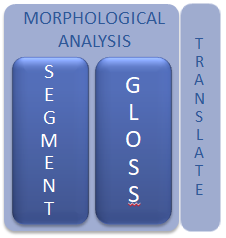
\includegraphics[width=0.3\columnwidth]{IGT.PNG}
\caption{Interlinearization. Words are segmented and morpheme boundaries are marked. Each morpheme is glossed (parsed). Finally, each sentence is translated in a language of wider communication to clarify how the morphemes compose meaning.}
\label{fig:IGT}
\end{center}
\end{figure}
 
In computational morphology, the two tasks, if both are attempted, are often tackled sequentially. First, the machine finds morpheme boundaries, then attaches labels. In a narrow sense, since a machine cannot make analytical decisions that a human can (though it can find complicated patterns and make predictions which may seem like analytical decisions), all computational morphology could be seen as annotation. However, some computational models have taken a tip from LDD workflow and united the two tasks. In some cases, this yields higher accuracy. It also allows the machine to go beyond annotation and ``learn a probabilistic model of morphotactics [rules about the ordering and co-occurrence of morphemes on a word]'' \cite[page 165]{cotterell_labeled_2015}.
Morphological segmentation and tagging should be distinguished from syntactic annotation, of which the most common type is part-of-speech (POS) tagging, but this distinction can be problematic because some POS tag sets such as the expanded set of Universal Dependency tags \cite{de_marneffe_universal_2014} include morphologically-marked syntactic features, such as number or grammatical case. In fact, ``morphological'' tag sets and ``morphological'' annotation could benefit from even more syntactic information \cite{cotterell_cross-lingual_2017}. LDD distinguishes morphological annotation from syntactic annotation even less strictly than computational linguistics. IGTs often include lexical categories (POS) and information related to syntax, phonology, and even non-verbal communication. The fact is that the divisions (morphology, syntax, phonology, etc.) are convenient for linguistic science but are not as clear in natural language. The division between morphology and syntax is more obvious in the relatively simple morphological structures that many high resource languages have, such as the fusional morphology of most European languages or the isolating morphology of Chinese languages. Both fusional and isolating morphologies use independent function words (e.g. prepositions, particles, etc.) rather than bound morphemes to express a significant amount of syntactic information. Even some more complex morphological structures, such as the non-concatenative, templatic Arabic, also expresses a fair amount of syntactic information with independent words. These strategies stand in contrast to agglutinative and polysynthetic morphology characterizing many low resource languages, which express most or all syntactic information by bound morphemes on the inflected word forms. 

\subsection{Morphological Paradigm Induction}
\label{paradigms}

The study of a language's morphology extends to the inference of the system of rules that dictate how morphemes build words and interact with each other. This inference is based on three assumptions \cite{durrett_supervised_2013}. First, within a lexical category lexemes inflect according to patterns that is dictated by a subsystem of rules. Russian nouns, for example, can be generalized into three simplified patterns of inflection, shown in Table \ref{tab:RuParadigm}. Lexemes that follow the same pattern are called inflectional classes (sometimes called ``declensions'' for nouns and adjectives and ``conjugations'' for verbs). Their patterns are sometimes called inflectional paradigms. Second, inflectional patterns are triggered by context and, therefore, the morphological rules dictating the patterns can be inferred from context. Descriptive studies look to phonology for the triggering context or else to both phonological structure and the semantic content of the lexeme. Computational models, due to the nature of their input texts, look to orthographic context. The third assumption is that a stem morpheme is inflected consistently. 

Understanding a language's morphology means discovering paradigms and identifying the inflectional class of each lexeme. A lexeme's inflectional class becomes a useful part of its dictionary entry. The inflectional pattern of a class is described in an inflectional paradigm which display either just the inflectional affix(es), as in Table \ref{tab:RuParadigm}, or a sample lexeme with all its inflected forms. Paradigm tables are featured in published grammatical descriptions and used for language learning. 

\begin{table}[ht]
\begin{center}
%\begin{adjustbox}{width=\columnwidth}
\begin{tabular}{c|cc|cc|cc}
\toprule
{} & \multicolumn{2}{c|}{\bf Class 1} & \multicolumn{2}{c|}{\bf Class 2} & \multicolumn{2}{c}{\bf Class 3} \\
{}	& \textsc{sg} & \textsc{pl}	& \textsc{sg} & \textsc{pl} & \textsc{sg} & \textsc{pl} \\
\midrule
\textsc{nom} & -a & -\textbari & \O & -\textbari & -\textsuperscript{j} & -i \\
\textsc{acc} & -u & -\textbari /\O  & \O/-a & -\textbari/-ov & -\textsuperscript{j} & -i/-jej \\
\textsc{gen} & -\textbari & \O & -a & -ov & -i & -jej \\
\textsc{dat} & -je & -am & -u & -am & -i & -jam \\
\textsc{inst} & -oj & -ami & -om & -ami & -ju & -jami \\
\textsc{prep} & -je & -ax & -je & -ax & -i & -jax \\
\bottomrule
\end{tabular}
\end{center}
\caption{Example of Inflectional Paradigms for Russian Nouns. The second row and leftmost column indicate the morphosyntactic features that each slot represents.}
\label{tab:RuParadigm}
\end{table}

These tables are challenging to induce from raw data. Within one language, inflectional classes are not always unique or regular, they may have overlapping patterns and isomorphic morphemes that result in ambiguous forms. For example, an Arapaho verb ending in \textit{-\'ot} might mean ``You alone do something to \underline{him/her/it}'' or it might mean ``You alone do something to \underline{them}.'' Some languages use suppletive forms that have no similarity in shape to their ``base'' form (e.g. English ``go'' vs ``went''). Field linguists can refer these difficulties to native speakers but machine inputs are typically limited to written texts sourced from published material.

\newcite{monson_paramorfinding_2007b} stated two guiding principles for paradigm induction. First, ``in any given corpus, a particular lexeme will likely not occur in all possible inflected forms''.  Even with a large corpus, attempts to recreate a paradigm as in Table \ref{tab:RuParadigm} will result in empty gaps. Language documentation best practice field methods encourages elicitation of inflectional paradigms in focused sessions---despite the subfield's emphasis on natural language---precisely because complete paradigms so rarely appear in natural language \cite{lupke_data_2010}. Certain inflectional forms will be much more common than others. In fact, for some lexemes, certain inflectional forms may never occur in spoken language even though they are grammatically possible \cite{silfverberg_encoder-decoder_2018}. It may be possible to find all inflectional forms of the most frequent lexemes, but frequent words may follow irregular patterns such as the English ``be'' verb. Therefore, paradigms need to be completed by inducing the patterns from several incomplete paradigms. The second principle is that inflected forms of a single lexeme will be similar. It is not always true---languages abound with exceptions where a word changes drastically during inflection (e.g. \textit{go} vs. \textit{went})---but it is a solid working assumption.  

Descriptive linguistics infer inflectional paradigms from annotated data. An ideal analysis strives to describe all possible patterns of inflection. Theoretically, this means that every inflectional form of every word needs to be examined, but in practice, paradigmatic patterns can be inferred fairly quickly and the linguist can then concentrate on matching lexemes to a paradigm and identifying irregularities. Analysis is often assisted by spreadsheets in computer programs such as Microsoft Excel.

Computational models have successfully induced frequent and regular paradigms with high accuracy even in low resource settings \cite{hammarstrom_unsupervised_2011,durrett_supervised_2013,ahlberg_semi-supervised_2014}. Most early work on computational morphological paradigm induction applied unsupervised learning to concatenative morphology \cite{goldsmith_unsupervised_2001,chan_learning_2006,monson_paramorfinding_2007b}. Supervised and semi-supervising models have been more recently applied on concatenative and non-concatenative languages \cite{dreyer_discovering_2011,durrett_supervised_2013}. ParaMor \cite{monson_paramorMinimally_2007a} is an example of an unsupervised model. It begins by searching the data for strings that resemble inflectional paradigms. It does this by identifying candidate ``suffixes'' in word-final substrings. A candidate suffix is a substring that is found at the end of many different words. The suffixes are refined into sets of partial paradigms. 

Inflectional paradigms induced by unsupervised learning has three flaws. First, a suffix might actually belong to multiple paradigms. The form of suffixes overlap between paradigms. For example, ``-s'' on an English word may mark noun plurality or it may mark third-person singular subject agreement in the present tense on a verb. Second, most candidate paradigms contain ``many fewer candidate suffixes than do the true paradigms'' \cite[page 903]{monson_paramorfinding_2007b}. This is a manifestation of Monson's first principle: induction from natural text leaves gaps because some inflected forms are rare or never used at all in natural speech. Third, some suffixes will inevitably be identified incorrectly; morpheme boundaries will be segmented at the wrong place. For example, the English word ``ally'' could be easily misidentified as a root ``al'' plus the adverbializing suffix  ``-ly''. ParaMor solves the first two flaws by leveraging Monson's second principle of consistency of form. It measures the similarity of word forms and uses that similarity score to cluster candidate suffixes into sets that appear on the same or similar roots. The third flaw is addressed by filtering paradigms. If a set has only a few suffixes, it is assumed this is due to spurious morpheme identification. So a number is chosen and any candidate partial paradigm with suffixes below that threshold are filtered out. 

Paradigm learning with supervised machine learning means at least partially complete paradigm tables are needed to train a model. A common source of inflectional tables is Wiktionary, a crowd-sourced online dictionary. Wiktionary contributors usually include an inflectional table for each entry. Sometimes, if known, the lexeme is identified with its paradigm or inflectional class. Some supervised learning has been applied to tasks related to paradigm learning but that are not direct attempts to identify a language's inflectional classes but focus instead on generating correct inflected forms. For example, \newcite{malouf_generating_2016} applied supervised deep learning in the form of recurrent neural networks to answer the Paradigm Cell Filling Problem (PCFP) \cite{Ackerman_partsand}, illustrated in Figure \ref{fig:PCFP}, which asks how new speakers infer the inflected forms of a lexeme when they have not seen all forms? Malouf et al.'s model took as input the ``base'' form represented as a one-hot vector and the morphosyntactic features tags of the inflected form to generate. For example, if the input is a representation of ``walk'' and the features tense = \textsc{pres}, person = \textsc{3}, number = \textsc{sg}, then the correct output is ``walks''. The model was successfully applied to Irish, Maltese, and Khaling [klr], as well as some major languages. One interesting observation was that regularization, which normally keeps the model from overfitting, was found to harm performance because the less frequent inflectional patterns look like noise. Regularization tends to guide the model away from those patterns, when it actually needs to learn them. \newcite{silfverberg_encoder-decoder_2018} also investigated the PCFP. With the same amount of input their results were very similar Malouf et al.'s but their model is more realistic for LDD. They do not use the lexeme, which, in morphologically complex languages, is rarely found in naturally-occurring texts. Instead, they trained on inflected forms, which could be extracted from a LDD corpus. Crucially, their input and output were actual strings, not numbers to represent the lexeme and one-hot features to represent the inflected form. This allows it to work on unseen forms. 

\begin{figure}[ht]
\begin{center}
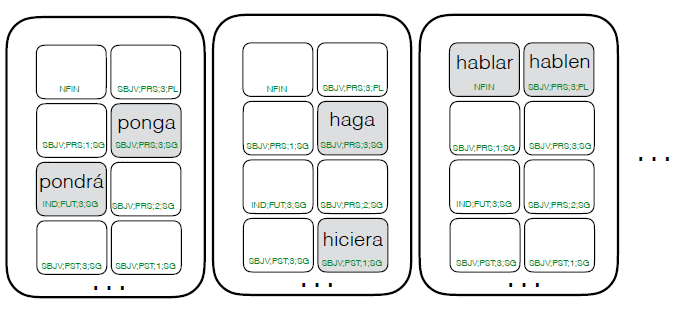
\includegraphics[width=0.7\columnwidth]{PCFP.PNG}
\caption{\newcite{silfverberg_encoder-decoder_2018}: Illustration of the Paradigm Cell Filling Problem with Spanish verb inflectional tables. If speakers are only exposed to such partially filled paradigms, how do they fill the missing cell with the correct form?}
\label{fig:PCFP}
\end{center}
\end{figure}

\newcite{kann_neural_2016} use a deep learning approach to morphological re-inflection. Re-inflection attempts to predict a correct inflected form from another form or from morphosyntactic tags or \textit{vice versa}. This is essentially the same task as the approaches to the PCFP, but without reference to the theoretical question, and therefore, is not compelled to limit the input: Kann et al. used completed inflection tables. Their approach does not learn inflectional patterns directly but it outlines possible first steps toward morphological paradigm induction in low resource settings. The model draws inspiration from the theoretical linguistic notion of principal parts \cite{finkel_principal_2007} which refers to minimal subset of forms that allow maximum predictability. This subset can be thought of as the smallest number of inflected forms needed to identify the lexeme's inflectional class. Kann et al. added encoders that incorporate multiple inflected forms, with the assumption that these multiple forms provide complementary information about a pattern and allows the model to predict a complete paradigm. Such ``multi-source'' learning performs better than a single data source by working around ``holes” in data. It can be applied to fully or only partially annotated data.

A similar approach can be applied to low resource settings \cite{ahlberg_semi-supervised_2014,ahlberg_paradigm_2015} using a small number of inflectional tables from Wiktionary which are similar to Table \ref{tab:RuParadigm} but include the whole word instead of the just the inflectional morphemes. With this data, groups of similarly behaving words were extracted from annotated data. Several of these groups were used to identify paradigmatic patterns.  As with Kann et al. the immediate goal is to predict the correct inflected forms of unseen words, but the generalized patterns used to make these predictions are basically inflectional paradigms. The patterns are discovered by abstracting the longest common subsequence in a word and clustering those abstract patterns with same or similar patterns. This is illustrated in Figure \ref{fig:LCS}\footnote{Acknowledgements to Mans Hulden and Ling Liu.}. The three parts of the longest common subsequence (LCS) \textit{rng} or \textit{swm} are extracted from the inflectional table on the left (step 1) and represented abstractly, in this case as \textit{x\textsubscript{1}} and \textit{x\textsubscript{2}}. The abstract symbols replace the longest common subsequence in every word form (step 2). In theory, the characters that remain, in this case \textit{i}, \textit{a}, \textit{u}, are the inflectional morphemes. Since the unique part of the each root morphemes is now represented identically, words with the same inflectional patterns will be identical and can be generalized into paradigmatic patterns (steps 3 and 4). It seems quite possible that exceptions or irregularities could be accounted for by collapsing similar patterns. The experiment was quite successful on some Indo-European languages (German, Spanish, Catalan, French, Galician, Italian, Portuguese, Russian), as well as Maltese and Finnish.

\begin{figure}[ht]
\begin{center}
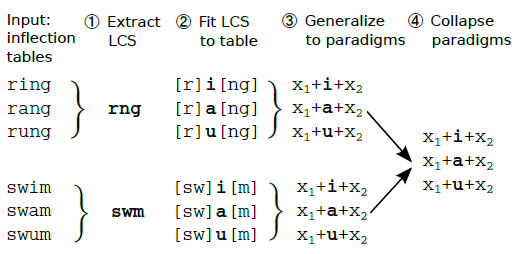
\includegraphics[width=0.7\columnwidth]{Ahlberg2015-LCS.PNG}
\caption{Ahlberg et al. (2015): Abstracting inflectional paradigmatic patterns from inflections and annotated data.}
\label{fig:LCS}
\end{center}
\end{figure}

Attempts at paradigm induction has contributed to computational morphology in low resource  contexts in a singular way: those attempting it have also attempted to estimate the smallest amount of data necessary to perform it with reasonable accuracy. \newcite{ahlberg_semi-supervised_2014} found that paradigms from the 20 most frequent inflectional classes cover 95\% of German word forms. \newcite{detrez_smart_2012}, who use hand-written rules to fill paradigm slots, started with complete inflectional tables and gradually dropped information from them. In the end, they found that one-two infected forms per paradigm are sufficient to achieve 90\% accuracy in English, Swedish, French, and Finnish. \newcite{silfverberg_encoder-decoder_2018}, using a neural model that learns from a small number of randomly chosen forms per paradigm table, found that two inflected forms gave about 85\% accuracy in Finnish, Georgian, Turkish and some Indo-European languages and three forms bumped the results over 90\% for all but Georgian nouns and Latvian verbs.

\section{Approaches to Computational Morphology}
\label{compMorph}

This section explores the exciting development of computational morphology and its application to low resource languages. The four major approaches are either  rule-based (finite state transducers) or machine learning approaches that induce models from texts. Machine learning strategies differ in whether the texts have been annotated completely (supervised), partially (semi-supervised), or not at all (unsupervised). Until the late-1990s and mid-2000s, the literature on computational morphology was dominated by finite-state machines \cite{kaplan_phonological_1981,koskenniemi_two-level_1983,beesley_finite-state_2003}. Gradually, machine learning started to become popular \cite{cohen_joint_2007,ruokolainen_comparative_2016}. Most early machine learning of morphology used unsupervised, probabilistic models \cite{roark_computational_2007}. Supervised approaches came later, due in part to computer memory limitations \cite{hammarstrom_unsupervised_2011}. Semi-supervised learning has also grown in popularity, due perhaps in part to ``the increased availability of machine-readable inflection tables'' \cite[page 18]{goldsmith_computational_2017}. 

Currently, supervised end-to-end neural networks, or deep learning methods, are dominating the field. Although deep learning approaches have achieved high results in many NLP tasks, they did not become popular until recently because they train more slowly than non-neural methods for some tasks \cite{cotterell_cross-lingual_2017} and require greater computing power. Significantly,  the models and methodology have greatly improved in recent years. More significantly, an important model for NLP, and morphology in particular, the sequence-to-sequence (seq2seq) model, was not developed until more recently. Unfortunately, deep learning models require expertise to customize. General linguistics training does not include computer programming and, as yet, few, if any, easy-to-learn graphic user interfaces exist. This still presents a practical hurdle to efficient NLP application in LDD.  

Computational morphological approaches have been tested on a growing number of languages since 2000 \cite{hammarstrom_unsupervised_2011}. The latest CoNLL-SIGMORPHON Shared Tasks \cite{cotterell_cross-lingual_2017,cotterell_conllsigmorphon_2018} indicate how this number has grown. Nevertheless, the task's list of 100+ languages is still small in comparison to nearly 6,000 remaining languages. Nor has the number grown in a representative way. The distribution is not proportional to language families or basic morphological types. As an example, the 2018 CoNLL-SIGMORPHON task included only one language classified as polysynthetic, and that language, Navajo, is often classified as agglutinative or fusional.

It is worth noting that comparing the performance of different approaches, and the different models within one approach, is not straightforward. Morphological analysis involves many small steps; if any one step is the basis for evaluation, the assessment changes. A predicted segmentation can miss the correct morpheme boundary by one letter or by many. Precision and recall can be calculated as a ``micro-average'' that is measured across all segmented boundaries or as a ``macro-average'' measured across all word forms \cite{ruokolainen_supervised_2013}. For the latter measure, the total count for precision, recall, and F1 measure could be based on types or on tokens. A word type count may obscure whether all types are handled identically. A word token count may make the model seem less accurate if one very frequent word is incorrectly parsed. Some evaluations may consider a parse correct when it produces one of all possible ambiguous parses; others may count a correct parse only when it is the right one in the given context \cite{ruokolainen_supervised_2013}. \newcite{virpioja_empirical_2011} surveyed these issues through five years of MorphoChallenges and found no solution to the varying details, but they concluded that an evaluation based on segmentation is the most simple, robust, and intuitive. Beyond the difficulties caused by varying standards of comparison, computational linguistics evaluates models in two ways. The first is indirect, or extrinsic evaluation, which evaluates the effect a model has on a complete NLP system. This is complicated and time-consuming and so rarely done. Direct, or intrinsic, evaluation is can be performed either automatically against gold standard, annotated data or manually by native speakers or domain expert linguists. \newcite[page 53]{virpioja_empirical_2011} dismiss manual evaluation because human expert decisions are ``subjective'' and ``the amount of work involved restricts its usage.'' This disregards the fact that any gold standard data was originally assembled with the same amount of human subjectivity and hard work. Such attitudes reveal the drawback of intrinsic evaluation. It sets a narrow focus on how a model performs competitively against other models on the same dataset, rather than how it performs across datasets or languages. 

\subsection{Finite State Transducers}

Finite state transducers (FSTs) are bidirectional, rule-based models that have successfully modeled linguistic patterns \cite{koskenniemi_two-level_1983,beesley_finite-state_2003,hulden_finite-state_2009}. They were the first computational model to successfully both parse and generate word forms \cite{goodman_generation_2013} (see Figure \ref{fig:bidir}). Since they easily represent regular relations between underlying and surface forms, moving left-to-right, they held early importance as a way to represent \newcite{chomsky_sound_1968}'s  rewrite rules \cite{karttunen_2005} and model the theory of two-level morphology.
\bigskip

\begin{figure}[ht]
\begin{center}
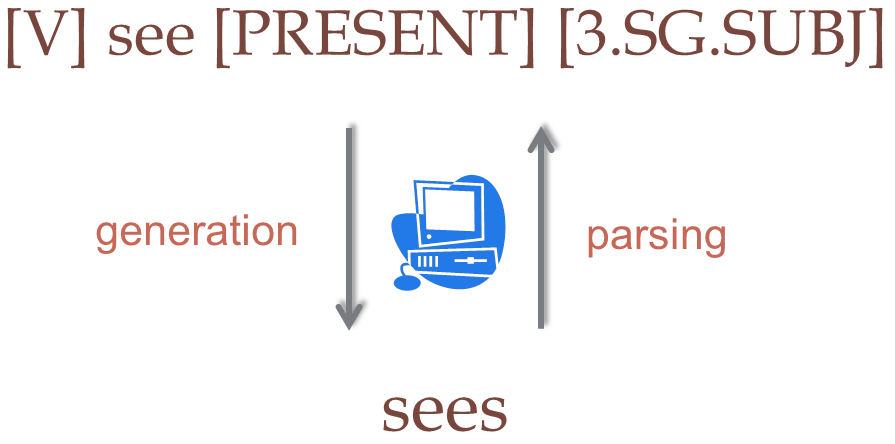
\includegraphics[width=0.5\columnwidth]{bidirectional.PNG}
\caption{A bidirectional computational morphological model generates an inflected word form from a stem and morphosyntactic tags and parses inflected words forms into stem and tags.}
\label{fig:bidir}
\end{center}
\end{figure}

FSTs are constructed in two steps. The first step specifies the lexicon and morphotactics in a finite-state lexicon compiler ({\it lexc}), illustrated in Figure \ref{fig:lexc}. This is where concatenative morphological rules and morphological irregularities are addressed. The second step implements morphophonogical rewrite rules. These rules apply changes in specified contexts, allowing the FST to move beyond simple concatenation of morpheme strings and generate well-formed inflected surface forms. For example, a rule would specify that the final letter in the Arapaho stem \textit{noohow} `see' transforms into a \textit{b} if a vowel-initial morpheme is suffixed after it.
\bigskip
\begin{figure}[ht]
\begin{center}
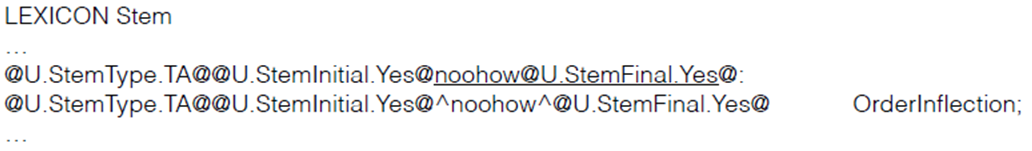
\includegraphics[width=0.95\columnwidth]{FSTlexicon.PNG}
\caption{A snippet of an Arapaho \textit{lexc} file for one stem morpheme \textit{noohow} `see'. The @ symbols surround flag diacritics that communicate how the rewrite rules should handle transformations unique to the stem's inflectional class or other exceptional morphophonological behavior.}
\label{fig:lexc}
\end{center}
\end{figure}

FSTs remain important to computational morphology. As recently as 2017, it was claimed that computational morphological learning methods are essentially still finite state methods \cite{goldsmith_computational_2017}, They have been found to be superior for many applications over a semi-CRF supervised machine learning model \cite{cotterell_labeled_2015}. With enough linguistic expertise and time for development, FSTs are capable of correctly analyzing any well-formed word in a language. However, FST “grammars” take significant effort to develop, maintain, and update \cite{durrett_supervised_2013,moeller_neural_2018}. Since the ``grammar" must be manually-constructed, FSTs require a thorough knowledge of the language and finite state machines, although in at least one case a FST morphological analyzer has been constructed from labeled inflection tables; it was, however, limied to inflectional morphology \cite{forsberg_learning_2016}.

FSTs work well with languages that have strong constraints on how each lexical category (POS) can be inflected, such as Arapaho, with its unique polysynthetic verb forms. But while the bulk of the FST can be developed relatively quickly with basic descriptive resources (e.g. the Boasian Triad), its reliance on language-specific lexicons and rules means that a full FST grammar needs a language that has been thoroughly documented and described. FSTs can be made to generalize to unseen forms, and if both descriptive resources and a language expert trained to construct the \textit{lexc} and rewrite rules are available, an FST can be a good solution for simple morphological modeling. However, FSTs do not help resolve ambiguity because they output all possible outputs instead of ranking them by probability given surrounding context. An FST's output is always correct but sometimes it more practical for downstream tasks to have one ``best guess''. FSTs cannot be used for active learning easily since they do not learn patterns from new annotated examples. These issues can be resolved with machine learning.

\subsection{Unsupervised Machine Learning}

Unsupervised (computational) learning of morphology (ULM) began as an attempt to prove American structuralism and Bloomfield's ''inductive generalizations,'' as well as a possible language acquisition model \cite{hammarstrom_unsupervised_2011}. ULM models attempt to induce morphological patterns from raw, unannotated texts. They take as input natural language data and, with as little supervision (i.e. parameters, thresholds, human intervention, model selection, etc.) as possible, outputs a ``description'' of the language’s morphological structure, according to \newcite{hammarstrom_unsupervised_2011}. However, their use of the word “description” is a bit misleading. What ULM produces is only a first step to morphological description in general linguistics. \newcite[pp. 33-34]{settles_active_2010} depicts ULM more accurately as exploiting the ``latent structure [in the data] alone to find meaningful patterns'' or features. It outputs the data organized ``in a meaningful way'', usually via a clustering algorithm that finds natural groupings within the data. 

According to \newcite{monson_evaluating_2008}, unsupervised morphological models have followed three main stages of development. Early unsupervised algorithms drew inspiration from Z. Harris \cite{harris_phoneme_1955,harris_morpheme_1967}, who extended a descriptive methodology pioneered by Bloomfield that focuses on what elements in a language can co-occur or not. Harris observed that phonemes do not co-occur unpredictably. The probability of the second phoneme in a word is dictate by the first, the third is dictated by the first two, and so on, illustrated in Figure \ref{fig:harris}. \newcite{harris_phoneme_1955} was the first to use character predictability to identify morpheme boundaries. Second, models inspired by Harris used the Minimum Description Length principle (MDL). At the third stage of ULM development, models began to leverage patterns akin to inflectional paradigms in order to find inflectional relationships between words and identify their affixes.

\begin{figure}[ht]
\begin{center}
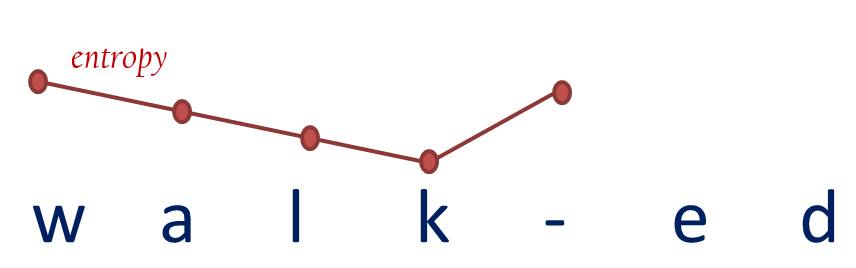
\includegraphics[width=0.5\columnwidth]{Harris-Entropy-image.PNG}
\caption{Harris' character predictability/entropy. In the word form ``walked" the possible letters that can follow the ``k are more than those that could follow the ``l'', so we predict a morpheme boundary.}
\label{fig:harris}
\end{center}
\end{figure}

MDL remains a leading method for unsupervised learning of morphology \cite{hammarstrom_unsupervised_2011}. It extends the Kolgomorov complexity that asks, in essence, ``What's the shortest (in terms of memory) computer program that generates some text?'' MDL simplifies this somewhat abstract question into a weaker but computable model. MDL-based approaches attempt to model the morphological structures by minimizing the memory cost of the input data and the model together. A proposed model encodes hypothesized morpheme strings with binary codes (essentially, a encoded lexicon or ``codebook'' of morpheme candidates) and replaces those strings with the codes whenever they appear in the input texts. The memory cost of the ``codebook'' and the encoded texts are calculated. The best morphological model is the one that where the cost of the ``codebook'' plus the encoded texts have the smallest possible memory cost (see Figure \ref{fig:MDL}\footnote{Generated at https://asr.aalto.fi/morfessordemo/}. Measuring the cost of the model inhibits overlearning and measuring the cost of the data, where the most frequent morphemes have the shortest codes, encourages frequent strings to be identified as repeated morphemes. Two downsides to MDL are that it provides no hint where the model should start looking for morpheme boundaries (what hypothesis it should start with) and it cannot it provide a coherent analysis across a whole language \cite{goldsmith_computational_2017}.

\begin{figure}[ht]
\begin{center}
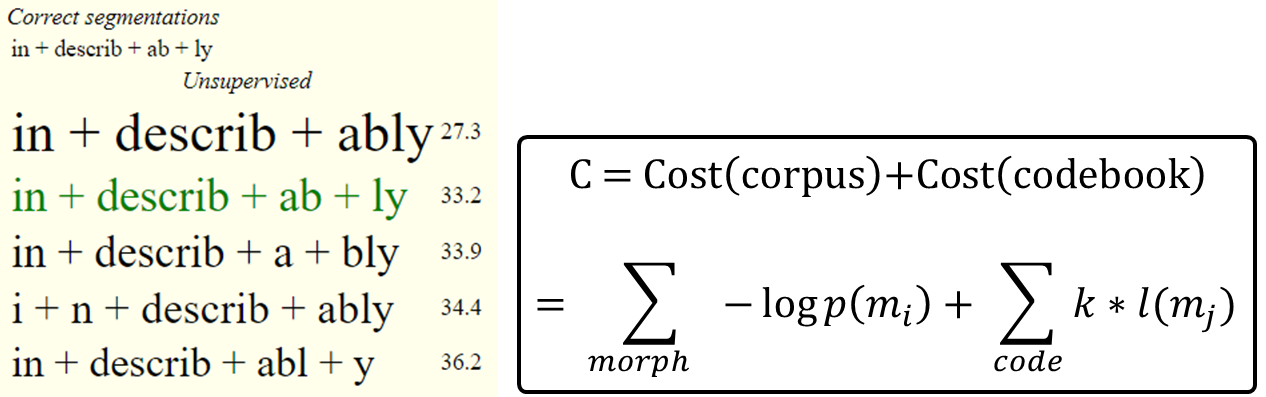
\includegraphics[width=0.9\columnwidth]{MDL2.PNG}
\caption{Minimum Description Length. The model makes random splits (marked by \textit{+} on left) in a corpus, resulting in strings of candidate morphemes, or ``morphs''. A ``codebook'' of binary codes that represent each morph is constructed so that more frequent ``morphemes'' are represented with shorter codes, reducing the average cost per morpheme. Then each occurrence of a morph in the corpus is replaced with its code. Finally, the total cost \textit{C} of the model (codebook) and the data (encoded corpus) is summed. On the left, this cost \textit{C} is shown next to the word for a model with various segmentations of ``indescribably''. The random splits that result in the lowest total cost is considered the correct morphological model. The ``wrong'' lowest score here demonstrates typical segmentation errors in unsupervised learning of morphology. The cost of the encoded corpus is calculated by summing the negative log likelihood of each morph's maximum likelihood \textit{$p(m_i)$} (i.e. the count of a morph's \textit{$m_i$} occurrences divided by the total number of morphs in the corpus). The codebook cost is calculated by multiplying the number of the bits \textit{k} needed to code a character by the character length of each morph \textit{$l(m_j)$}. }
\label{fig:MDL}
\end{center}
\end{figure}

Leading MDL-based models are Linguistica \cite{goldsmith_linguistica:_2000,goldsmith_unsupervised_2001} and the Morfessor family of algorithms \cite{creutz_unsupervised_2005a,creutz_unsupervised_2007}. Linguistica is a foundational work in ULM that attempts to discover “signatures”, shown in Figure \ref{fig:signatures}, which are sets of affixes somewhat akin to inflectional paradigms. Even though it is unsupervised, Linguistica needs to set an affix length limit and this requires at least enough knowledge of the language’s morphology to make a hypothesis. The latest version, Linguistica 5 \cite{lee_linguistica_2016}, attempts to make ULM more accessible by including a graphical user interface and an open-source, modular Python library. The library is meant to extend the model beyond morphology, taking syntactic context into account \cite{nicolai_morphological_2017}. Morfessor \cite{creutz_unsupervised_2005a,creutz_inducing_2005b,creutz_unsupervised_2007} attempts to identify the most likely ``morphs'' (candidate morpheme strings) and the most likely morpheme boundaries. Like many unsupervised models, it builds a morph lexicon. Relying on a lexicon of morphs reduces a model's cross-linguistic adaptability because the lexicon is specific to each language. The Morfessor model is built on two parameters that require some hypothesis about the language's morphology: ``(i) our prior belief of the most common morph length, and (ii) our prior belief of the proportion of morph types that occur only once in the corpus'' \cite[page 281]{creutz_unsupervised_2003}. Compared to Linguistica which is less eager to split words, earlier versions of Morfessor used Recursive MDL which tended make too many segments, but later versions of Morfessor stand somewhere in between early Morfessor and Linguistica in terms of segmentation accuracy \cite{creutz_unsupervised_2003}. 

\begin{figure}[ht]
\begin{center}
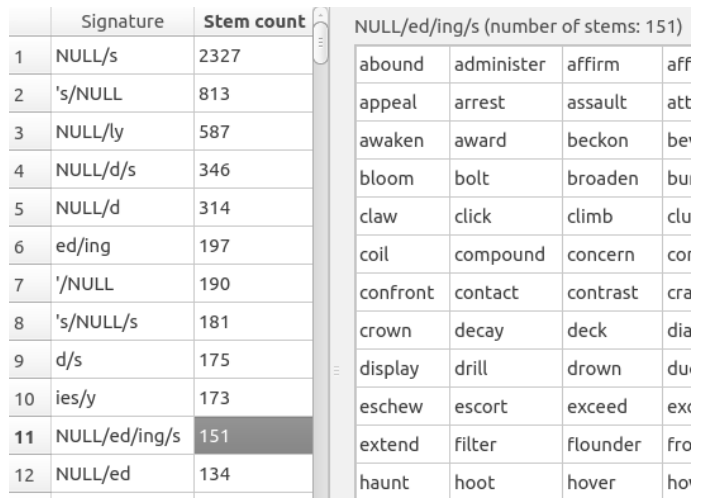
\includegraphics[width=0.5\columnwidth]{Linguistica5-signatures.PNG}
\caption{Screenshot of Linguistica 5. The column on the left displays hypothesized ``affixes'' that were found in complementary distribution on ``stems'', one group of which is displayed on the right.}
\label{fig:signatures}
\end{center}
\end{figure}

ParaMor is another unsupervised algorithm \cite{monson_unsupervised_2004,monson_paramorMinimally_2007a,monson_paramorfinding_2007b,monson_evaluating_2008}. Like Linguistica, it exploits patterns in the data similar to inflectional paradigms, but unlike Linguistica, it allows multiple segmentations per word. Paramor treats paradigm induction and segmentation separately but it does not address morphophonology as well as Linguistica. It requires more data but not as much memory. \newcite[page 49]{monson_evaluating_2008} claim that Paramor’s unsupervised induction of morphology could facilitate quick development of morphological learners for LRL, but they refrain from explaining how the system, which requires a significant amount of data, could do this.

Most ULM approaches are biased towards a certain affixing pattern or morphological type. Linguistica and ParaMor are tuned to suffixing morphology. Morfessor is better at prefixing+suffixing languages than the other two, but Linguistica does better with suffixing-only languages. All three are most suitable to agglutinative languages but also assume a small number of morphemes per word, often only one prefix/suffix. This does not bode well for morphologically complex languages. 

In theory, unsupervised models are the most exciting and attractive for LDD because they do not require costly data annotation. In fact, an early vision for ULM was to support language technology for minority language communities. This idealistic aim has not materialized because successful ULM demands ``a sufficiently large set of unannotated words in electronic form'' \cite[page 92]{ruokolainen_comparative_2016}. Languages that lack a basic morphological analysis generally lack the amount of raw data that accurate ULM requires. ``Sufficient'' data for unsupervised learning is in the order of a hundreds of thousands or a million words \cite{rocio_detection_2007}. A small corpus is defined as 1,000-100,000 words \cite{kirschenbaum_unsupervised_2012}. Since LRL includes well-documented languages, sometimes obtaining sufficient data may be simply a matter of digitizing existing literature, but for most, a limited written history means that texts must be first recorded orally and then transcribed before this a small corpus is usable. Although language documentation aims to generate a great deal of minimally annotated data \cite{himmelmann_documentary_1998,lehmann_documentation_1999}, LDD projects rarely produce even a 100,000 words and the transcribed portion tends to be much smaller.  Despite this, the claim is still being made that ULM methods, ``provide an inexpensive means of acquiring a type of morphological analysis for low resource  languages'' \cite[page 92]{ruokolainen_comparative_2016}. Another drawback is that unsupervised methods are less accurate than other machine learning approaches. \newcite{soricut_unsupervised_2015} were able to overcome this drawback, at least for some Indo-European languages by using unsupervised word embeddings (word meanings represented in vector space). However, even if word embedding increase accuracy, it is an open question whether they address the large data requirements since successful word embeddings are also built with large amounts of texts. 

\newcite{goldsmith_computational_2017} raise other problematic issues. For example, unsupervised approaches have to start with some assumptions about a language's morphology. Should we start with random parameters or should we use knowledge about the target language? The latter is the most efficient, but using prior linguistic knowledge, as Goldsmith, Lee, and Xanthos and \newcite{palmer_computational_2010} insinuate, means the approach is not truly unsupervised. It also makes ULM even less attractive for under-described languages. With such languages, we can presumably hypothesize from related or geographically adjacent languages, but this opens another question that is not clearly addressed in the literature: how well do current ULM methods transfer across languages, and can we even measure this reliably? This cannot be addressed until ULM models have been tested against a wider range of languages. Currently, English is the \textit{de facto} language in ULM \cite{palmer_computational_2010}. The tension between expanding computational models to a wider range of languages and the prohibitive cost of data to test and evaluate the models will continue to influence the development of computational linguistics unless  better data production methods are devised.

Although unsupervised machine learning is most suitable to resource-rich languages, ULM has been applied in low resource contexts. \newcite{palmer_computational_2010} incorporated unsupervised morphological segmentation as a first step towards semi-automated IGT production (interlinearization) in Uspanteko [usp], a Mayan language of Guatemala with some 4,000 speakers \cite{simons_ethnologue:_2018}. Words were assumed to be morphologically related if they were orthographically similar. Affix candidates were generated by assuming stems are longer than affixes and then filtering for statistically significant co-occurrences. \newcite{moon_unsupervised_2009} also applied ULM to Uspanteko with a method that assumed suffixation only and, most notably, incorporated awareness of document boundaries when generating and clustering candidate morphemes. This technique assumes spelling is likely to be consistent within a document but vary across documents. Considering that minority languages may not have a standardized orthography and transcribers may have little formal education in the language, this is a simple yet very practical twist on the “one sense per discourse” effect used in computational semantics which observes that if a polysemous word such as ``saw'' appears more than once in a document all occurrences are highly likely to express the same sense \cite{gale_one_1992}. Document boundary awareness assumes one inflectional paradigm per stem per document; that is, a morpheme that may belong to two lexical categories is highly likely to appear as only one within a single document. This technique reduces noise and improves results over Morfessor and Linguistica (for English). Remarkably, the performance degrades when the corpus size is increased, perhaps because of increased noise from spurious candidate morphs. \newcite{kirschenbaum_unsupervised_2012} applied ULM to a corpus of Kilivila [kij], an Austronesian language of Papua New Guinea with 20,000 speakers \cite{simons_ethnologue:_2018}. Inspired by \newcite{schone_knowledge-free_2000} and \newcite{Baroni02unsuperviseddiscovery}, they identified morphologically related words by orthographic similarity and a context co-occurence vector. They claim that the method prefers languages with infixes but it is unclear how they determined this with only one language. 

\subsection{Supervised Machine Learning}
\label{sec:supervised}

Supervised learning of morphology means that models are trained on gold standard annotated data rather than unannotated raw texts. It requires significantly less data than unsupervised learning. However, the data must be annotated. Annotated data makes supervised machine learning qualitatively different than unsupervised learning. Unsupervised learning clusters underlying patterns or features which may facilitate human analysis and description of the data. Supervised learning is trained on data that has already been analyzed and labeled. It learns the labeling and generalizes it, predicting, of with high accuracy, what labels unseen samples should have. 

The best performing non-neural supervised model for sequence prediction tasks such as morphological analysis is conditional random fields (CRF) \cite{lafferty_conditional_2001,muller_efficient_2013,ruokolainen_comparative_2016}. A CRF is a sequence classifier that considers the whole sequence when making a prediction for each symbol in the sequence. In morphology, CRFs can work as boundary detection (segmentation) and labeler. According to \newcite{ruokolainen_comparative_2016}, discriminative learning methods such as CRF are better than generative models because they optimize the accuracy of segmentation boundaries and generalize better to unseen forms, assuming they have sufficient training data. A discriminative model's strength lies in its ability to define features beyond the previous label and allow arbitrary weights. CRFs apply logistic regression which allows it to make generalized predictions from arbitrary and possibly dependent features \cite{ruokolainen_supervised_2013}. 

A CRF can look at a number of features as it makes a prediction. A feature function input for a (linear-chain) CRF in morphological labeling might be 1) a whole word segmented into morphemes, 2) the position of the current morpheme in the word, and 2) the label of the previous morpheme. Each feature is weighted during training and, with these weights, labeling predictions are scored over the whole sequence, then transformed into a probability. For example, in a segmentation task where the previous word is ``am/is/are/was/were'', if the target word ends in ``ing'' and a weighted feature is the previous word the CRF might give a high weight to ''-ing'' as a separate morpheme. In labeling, the CRF might decide a word-final ``s'' marks a plural noun and not the 3rd person singular simple present tense by highly weighting the POS tag of the stem. However, the quality of the results relies heavily on the choice of features. This could be a drawback for under-described languages, because if little linguistic description is available then how does one know which linguistic features are optimal? Fortunately, CRFs have been shown to perform reasonably well using primarily language-independent features (i.e. surrounding substrings) \cite{ruokolainen_comparative_2016,moeller_automatic_2018}, including a model trained on approximately 3,000 words of Lezgi [lez], an agglutinative Nakh-Daghestanian language with about 600,000 speakers \cite{simons_ethnologue:_2018}. However, it is not  clear if the performances were more dependent on language-specific or task-specific features.

Supervised (and semi-supervised, see section \ref{semi-supervised}) learning requires less data and almost always achieves better results than unsupervised learning \cite{ruokolainen_supervised_2013} and, therefore, seems more promising for LDD. However, it may be necessary to augment textual data with other descriptive resources such as grammars and dictionaries since the size of annotated LDD corpora are still ``inadequate for supervised learning'' \cite[page 18]{duong_natural_2017}. This is not an impractical expectation for LDD since descriptive linguists traditionally result in the Boasian triad, described in Figure \ref{fig:Triad}.

\begin{figure}[ht]
\begin{center}
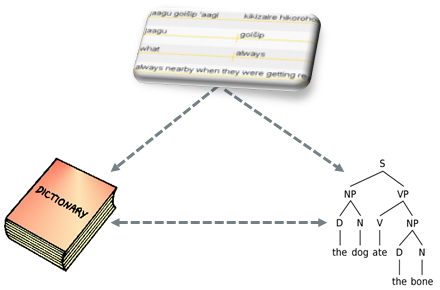
\includegraphics[width=0.7\columnwidth]{Triad.PNG}
\caption{The Boasian Triad. Traditionally, linguists working in new languages concentrate on producing a corpus of interlinearized texts, a grammar, and a dictionary. The interlinearization is a pre-step and feeds directly into the other two steps.}
\label{fig:Triad}
\end{center}
\end{figure}

\subsection{Supervised Neural Networks or Deep Learning}
\label{sec:NN}

 Neural networks (NN), or deep learning, is a family of machine learning techniques that builds layers of perceptrons that can learn complex patterns. Vector representations of the data are received by an input layer, fed into and transform in ``hidden'' layers then arrive at the output, or activation, layer.  Each unit in each layer is connected to each unit in the adjacent layers. The connections are represented by learnable weights; the higher the weight the more influence a unit has on the result. Since deep learning is supervised\footnote{Deep learning morphological segmentation has been performed on unsupervised texts with some success \cite{wang_morphological_2016}} the weights are adjusted via stochastic gradient descent with backpropagation using ``feedback'' from annotated data. Many flavors of deep learning exist and different models work best for different tasks. Recurrent neural networks (RNN) \cite{Elman91} with long short-term memory gates (LSTM) \cite{Hochreiter_1997} are currently considered state-of-the-art for most sequence-based NLP tasks. RNNs may have one layer and recurrently add its output to next input and feed that into that layer. Many may have multiple layers and the recurrence occurs only for each time step in the network. This works as a feedback loop. RNNs can input and output sequences of values. A probabilistic prediction of the next item in a sequence is conditioned on the entire sequence of transformations and previous predictions in each time step. Unfortunately, the typical deep learning problem of vanishing gradients, or decay of information through time, is much worse for RNN. That is why the LSTM memory gate is so important. The LSTM decides how much of the previous output should feed into the next recurrence and how much should be ``forgotten''. Dropping ``forgotten'' information from the calculation allows RNNs to propagate the gradients much more efficiently back through the entire sequence of time steps.
 
 \begin{figure}[ht]
\begin{center}
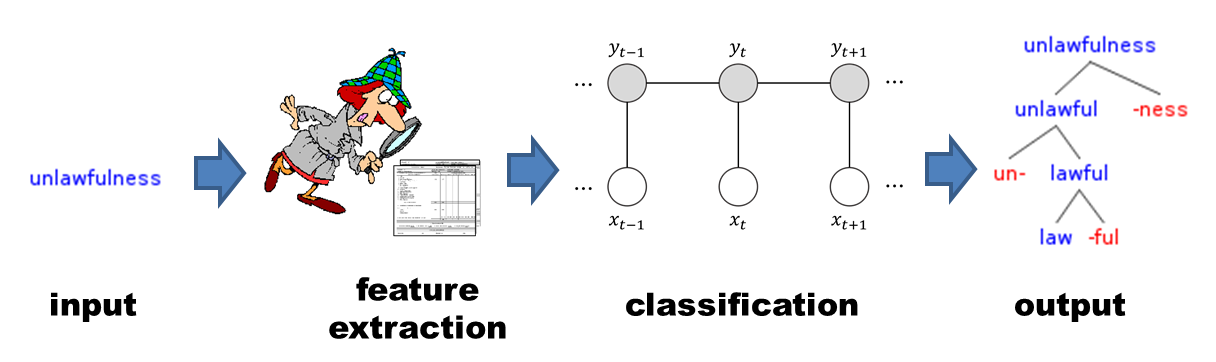
\includegraphics[width=0.95\columnwidth]{Features-ML.PNG}
\caption{Classical machine learning. In feature-based models a human expert must analyze and define optimal features from the data. A CRF usually uses gradient descent to assign weights to those features during training. A discriminative model such as Conditional Random Fields, can assign arbitrary weights.}
\label{fig:Features-ML}
\end{center}
\end{figure}

\begin{figure}[ht]
\begin{center}
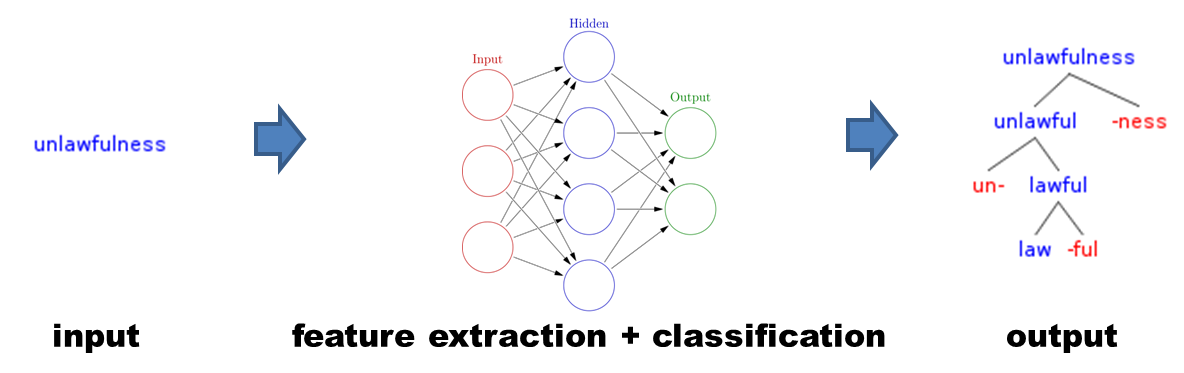
\includegraphics[width=0.95\columnwidth]{DL.PNG}
\caption{In deep learning, hidden layers create intermediate representation of the data. These essentially serve the function of feature engineering in non-neural machine learning.}
\label{fig:DL}
\end{center}
\end{figure}

In morphology, deep learning methods can be used to classify, generate sequences, or to performs sequence-to-sequence mapping. Classifiers classify data points into categories or classes. A data point might be a morpheme and the classes morphosyntactic tags. 
The hidden layers feed into a final logistic function layer (i.e. softmax) that outputs a prediction of each possible class as a probability between 0 and 1. Morphological generation produces fully inflected forms from morphosyntactic or contextual information \cite{cotterell_conll-sigmorphon_2017} or completes morphological paradigms \cite{malouf_generating_2016}. Currently, the strongest generator models use an encoder-decoder, also known as sequence-to-sequence (seq2seq), architecture of a RNN \cite{sutskever2014,kann_neural_2016}. Encoder-decoders map one sequence to another of a different length by encoding an input sequence of symbols (e.g. the letters of a word) and decoding it as another sequence of symbols (e.g. morphosyntactic tags). Encoder-decoders are also state-of-the-art for morphological tagging \cite{heigold_extensive_2017}, morphological segmentation (including low resource settings) \cite{kann_fortification_2018}, and morphological paradigm completion \cite{cotterell_conllsigmorphon_2018}. 

Until recently, neural networks were considered to have the same drawback as unsupervised learning: large amounts of training data for good results \cite{cotterell_conllsigmorphon_2018}. While it is true, for example, that top performing neural networks generate inflected forms with less than 60\% average accuracy when given only 100 training examples, results can increase significantly (over 85\%) when trained on 1,000 and 10,000 examples (up to 96\%) \cite{cotterell_sigmorphon_2016,cotterell_conll-sigmorphon_2017,cotterell_conllsigmorphon_2018}. Improved results cannot always be accomplished by the tuning tricks common with normal data sizes. For example, adding hidden layers can actually reduce accuracy with smaller amounts of data \cite{cotterell_conll-sigmorphon_2017}. Low data settings require unique techniques that include adjusting the model, training an intermediate step, and artificially augmenting the data. As an example of adjusting the model, \newcite{sudhakar_experiments_2017} found that using a gated recurrent unit (GRU) to control access to previous states in the RNN, rather than the NLP state-of-the-art LSTM, gave better results with up to 1,000 training examples. Successful intermediate steps in morphology include training the model to make edits to a string instead of decoding a new sequence, so, for example, the model learns an INSERT operation will generate ``runs'' from ``run''  (these models use some sort of alignment to reduce the number of edit operations between related forms) \cite{makarov_align_2017,makarov_uzh_2018}. Other successful intermediate steps include the whole sentence where an inflected form is or should used or train a model to first produce abstract underlying forms (e.g. ``impossible'' $\rightarrow$ ``in-possible'' $\rightarrow$ ``\textsc{neg}-possible'') the final inflected or parsed form \cite{liu_morphological_2018,moeller_improving_2019}. In recent CoNLL-SIGMORPHON submissions, participants found that these, and other new techniques considerably outperformed the state-of-the-art encoder-decoder baseline \cite{bergmanis_training_2017}. These successes suggests that developing unique techniques for morphological analysis of low resource languages is a promising area for exploration. A few of these techniques are discussed further in section \ref{augment}. 

\subsection{Semi-Supervised Machine Learning}
\label{semi-supervised}

Unsupervised learning may require less costly annotated data and supervised training may beat unsupervised training in accuracy but combining the two may be the best of both worlds. Semi-supervised, or minimally supervised, learning combines annotated data with a larger set of unannotated data when available annotated data is not adequate to effectively train a supervised model \cite{kohonen_semi-supervised_2010,poon_unsupervised_2009}. Like unsupervised learning, semi-supervised learning exploits the underlying structure of raw texts, but with the goal of improving the machine’s predictions, rather than discovering new ones \cite{settles_active_2010}. 

Semi-supervised learning has been widely researched for computational morphology and a wide variety of techniques have been employed \cite{ruokolainen_comparative_2016}. Some ULM algorithms, such as Morfessor Baseline, have proven adaptable to semi-supervised learning \cite{kohonen_semi-supervised_2010}. \newcite{dreyer_discovering_2011} used a ``mostly unsupervised'' method that employs a generative probabilistic model and 10 million unannotated words. It does POS-tagging, segments and tags morphemes, and identifies candidate inflectional paradigms. \newcite{ahlberg_semi-supervised_2014} predicted general paradigmatic patterns using longest common substrings and some unannotated data (LCS) (see section \ref{paradigms} for more details). The latter two models presuppose a few completed inflectional paradigms which are provided by native speakers either directly, or as computational linguists tend to prefer, through the indirect means of an expert who pre-processes the data or through crowdsourced resources such as Wiktionary.

While semi-supervised learning was early praised for its greater effectiveness and practicability, real applications were rare well into the late 2000’s \cite{druck_reducing_2007}. One reason may be that, like unsupervised learning which requires some initial hypothesis, many semi-supervised models make strong assumptions about the data. These assumptions may hold true in pre-processed datasets but ``tend to be violated in real-world data'' \cite[page 1]{druck_reducing_2007}. In addition, unannotated and annotated data cannot be simply combined together. Annotated data has to be weighted so that the larger, unannotated part does not overwhelm it. Overall, results in semi-supervised learning ``strongly suggest that it is crucial to use the few available annotated training instances as efficiently as possible before…incorporating large amounts of unannotated data'' \cite[page 35]{ruokolainen_supervised_2013}. 

Semi-supervised learning is promising for LDD because even though small amounts of annotated data are ``easy to get by manual annotation'' \cite[page 49]{virpioja_empirical_2011}, typical documentation corpora are only partially annotated. However, the results suggest that all available descriptive data for LRL should be exploited as much as possible before relying on unsupervised data. This heavy dependence on annotated data still poses a challenge \cite{andrews_bayesian_2017}. 

\section{Exploiting Resources}
\label{resources}

This section explores ways to improve results for some of the approaches discussed in section 2 when applied in low resource contexts. The high cost of annotating texts or manually constructing FSTs may be prohibitive,  and even though supervised and semi-supervised methods requires less data than unsupervised or neural network models, they still need significantly more data than is typically available for low resource languages. ``Understanding the available resources is the first step in building a natural language processing framework for a target low resource language'' \cite[page 13]{duong_natural_2017}. The spotty nature of LDD data necessitates using whatever resources are available \cite{palmer_semi-automated_2009}. This section present some techniques to exploit available resources other than textual data, such as artificially generated ``textual'' data, descriptive linguistic knowledge, and resources in other languages. 

\subsection{Non-Textual Resources}

Even though annotated textual data is scarce for most languages, many have been described to some extent and some linguistic resources exist for them. In practice, language documentation projects are rarely undertaken (and more rarely funded) except to support descriptive analysis and publication \cite{thieberger_using_2012,austin_language_2014,vallejos_integrating_2014,thieberger_assessing_2016}. Describing a language's morphological structure is relatively easy \cite{roark_computational_2007} and linguists tend to tackle it in the first stages. Minimally, a few inflectional paradigms can be easily elicited in a language documentation project. The bulk of a language’s morphology is described in structured data. Structured data might be any organized or pre-processed data that is not a naturally occurring text, such as inflectional tables or word lists.

Crowdsourced websites such as Wiktionary sometimes have inflectional tables for LRL. \newcite{cotterell_labeled_2015} successfully exploit spell checkers and Wiktionary to train a semi-supervised model. \newcite{ahlberg_semi-supervised_2014} use publically available inflection tables with a feature-based Support Vector Machine (SVM) to classify unseen lexemes into inflectional classes. \newcite{durrett_supervised_2013} also exploit Wiktionary for inflectional tables as the supervised part of a semi-supervised model. They claim that this allows their model to ``extend to other languages [with inflectional tables in Wiktionary] without change'' but it is to be expected some of the 150 or so languages on Wiktionary have very few tables. 

If data is thoroughly annotated, computational morphology can improve results from labeling that are not strictly morphological in nature. For example, \newcite{muller_efficient_2013} reduced CRF training time by performing a coarse POS-tagging then fine-grained morpheme tagging. The POS-tagging leaves the algorithm with fewer possible tags to process for each sample. 

Exploiting non-textual resources does not always improve results. Semi-supervised learning with a discriminative sequence learner like a CRF performs worse when non-textual resources are integrated because the external resources receive undue weight. \newcite{andrews_bayesian_2017} claim that models, such as a Maximum Entropy Hidden Markov Model, that generate a lexicon are less likely to degrade in performance because the lexicon essentially acts as an external resource and does not compete with the annotated corpus. 

\subsection{Transfer and Joint Learning}
\label{transfer}

Transfer and joint learning share a common big idea. They attempt to improve computational models by ``borrowing''. Transfer learning borrows the success of other models. Joint learning borrows information from other areas. 

Generally speaking, transfer learning assumes that what succeeds in one task will work well on another and it attempts to transfer that success. Transfer learning can be applied in semi-supervised and unsupervised learning \cite{duong_natural_2017}. When the task involves generalizing to another language, it often referred to as cross-lingual learning instead of transfer learning. Examples of cross-lingual learning are applying a successful morphological model to a new language or re-purposing annotated tags by aligning words across languages \cite{duong_natural_2017}. Generalizing across languages works better when a model is trained on more than one language. \newcite{kann_fortification_2018} found that single segmentation model trained simultaneously on four related polysynthetic languages performed as well as, and sometimes better than, single language models.

\newcite{baumann_using_2014} applied transfer learning principles by using an English word list to identify affixes in unlabeled data of Tagalog [tgl] and Zulu [zul], low resource languages (but clearly not endangered -- both have over 20 million speakers) spoken in the Philippines and South Africa respectively. The strategy was motivated by the realization that many low resource languages are spoken in multi-lingual contexts and have borrowed vocabulary from more economically powerful languages. A word list in that language identifies some root morphemes. Splitting substrings from these roots provides a list of prefixes and suffixes. With some knowledge of the language's morphological patterns, it was even possible to identify infixes in Tagalog. However, the strategy does not do well when a word has multiple affixes. 

Transfer learning is promising for low resource languages but it has its limitations. When RNNs performed cross-lingual morphological tagging on 18 languages from four language families, the conclusion was informative but perhaps unsurprising to those familiar with linguistic typology---the closer the languages' relationship, the more accurate were the results \cite{cotterell_cross-lingual_2017}. The precise correlation between linguistic genetics and results in transfer learning is largely unexplored \cite{buys_cross-lingual_2016,cotterell_cross-lingual_2017}, although interest is growing and new experiments are forthcoming \cite{sigmorphon2019}.  It is still not clear, for example, whether morphological structure or phonological (orthographic) similarity is a stronger factor. It \textit{is} clear that the amount of morphologically marked information common across languages influences results, so if a word ``in the source language does not overtly mark a grammatical category [that is marked] in the target language, it is nigh impossible to expect a successful transfer'' \cite[page749]{cotterell_cross-lingual_2017}. Transfer learning shows sharply the difficulties in paradigm induction.  Paradigms do not generalize across languages. Each language has its own unique ``layout'' for classes within each lexical category and these can differ considerably even in closely-related languages.

Since transfer learning can potentially overcome deep learning’s data hunger, discovering how to improve deep learning results in when transferring from high resource  to low resource settings would be ``a boon for low resource computational linguistics'' \cite[page 752]{cotterell_cross-lingual_2017}. \newcite{duong_natural_2017} points out that automatic projection of annotation (specifically, POS-tagging, noun phrase chunking, and dependency parsing) between high and low resource languages admits error at multiple points. The results have to be corrected or adjusted. Any projection-based method requires some seed data to perform well \cite{buys_cross-lingual_2016}, so one question ripe for exploration is how much data does the low resource target language need to balance a high resource source language's greater data? \newcite{cotterell_cross-lingual_2017} claim only a “small amount of annotation” is required; but they also claim the necessary annotation should not take too long. Conspicuously, they refrain from defining “small amount” and “not too long”. 

Joint learning trains simultaneously on different types of linguistic information. For example, since segmentation and tagging are generally separate task in computational morphology, training a semi-CRF to do both tasks would be considered joint learning \cite{cotterell_labeled_2015}. It is based on the intuition that one type of linguistic knowledge (e.g. syntax) can improve results in another domain (e.g. morphology), and vice versa \cite{goldsmith_computational_2017}. One of the earliest joint learning attempts was \newcite{schone_knowledge-free_2000}'s incorporation of semantic, orthographic, and syntactic information into unsupervised learning of morphology. The semantic information came from Latent Semantic Analysis which represents meanings as patterns of words that appear together in text, for example ``morphology'', ``morpheme'', ``inflection'''. Semantic information helped avoid the typical unsupervised segmentation error (e.g \textit{all-y} instead of \textit{ally}). It was supplemented by the probability of two affixes alternating on one ``stem'', which was calculated using orthographic information. Syntactic information was derived from the frequency of words that occur around pairs of possibly related inflected forms. The output was ``conflation sets'' which are paradigm-like groups (e.g. ``abuse'', ``abused'', ``abuses'', ``abusing'').
 
Since morphology carries a great deal, and in some languages most, syntactic information, syntax is important information for morphological analysis. Joint learning of syntax and morphology can be as simple as incorporating POS tags as features or extending POS tagging methods to morphological tagging \cite{buys_cross-lingual_2016,cotterell_cross-lingual_2017}. Syntax can also be incorporated into supervised learning by clustering words with similar final substrings which serve as a proxy for grammatical agreement and are assumed to indicate lexical categories \cite{lee_modeling_2011}. Successful joint learning of semantics and morphology has used the semantic information in word embeddings \cite{soricut_unsupervised_2015}. 

Joint learning in low resource settings has been successfully applied using information commonly produced by LDD projects \cite{palmer_semi-automated_2009,moeller_automatic_2018}, particularly POS tags.

\subsection{Data Augmentation}
\label{augment}

Another ``resource'' to exploit is artificially generated data to augment naturally occurring textual data. \newcite[page 38]{bergmanis_training_2017} found that the ``main benefit of the various data augmentation methods is providing a strong bias towards … regularizing the model, with a slight additional benefit obtained by learning the typical character sequences in the language." \newcite{kann_fortification_2018} found that with data augmentation a neural model can outperform Morfessor and match CRF accuracy. The success of these methods suggests that data augmentation may be a fruitful area of experimentation for applying neural models in low resource settings.

The most successful data augmentation strategies in low resource settings bias an encoder-decoder model to copy strings \cite{bergmanis_training_2017,kann_fortification_2018,makarov_align_2017,makarov_uzh_2018}. For example, \newcite{bergmanis_training_2017} and \newcite{kann_fortification_2018} auto-encode (train a model to output a string identical to the input) words from the training corpus. Their performance varied between languages, perhaps due to how well a language’s morphological features were represented in the small training datasets, but \newcite{bergmanis_training_2017} found this method performed better than transfer learning and \newcite{kann_fortification_2018}, who refer to the approach as ``multi-task learning'', found it superior to \newcite{silfverberg_data_2017}'s strategy of replacing common substrings in the test data with random strings from the training data.  Simplistically, we might assume that copying ``base forms'' (e.g. ``run'') would work well for morphologically simple languages that add few affixes to the base form, but the foundation of morphological analysis is the systematic patterns of inflection which means that all languages tend to repeat identical or very similar substrings across morphologically related forms. 

\section{Computational Morphology for Language Documentation and Description}
\label{CLLDD}

Computational linguistics has a solid history in morphology and success in low resource contexts is increasing. Unfortunately, general linguistics has witnessed little evidence of this success. Very little, if any, computational models have been applied to basic morphological analysis and annotation, which stands as a bottleneck in production of new and accessible language data \cite{holton_developing_2017}. This is doubly unfortunate because more data is vital resource in both general linguistics and natural language processing. This section describes the bottleneck and outlines how it can be addressed right now by integrating some of the machine learning models and techniques for exploiting other resources that are described in this paper. It then predicts how going beyond strategies discussed in this paper could even more quickly increase new data so that it becomes accessible for research and development in both fields.

\subsection{Interlinearization: A Bottleneck}
In the typical LDD workflow morphological analysis takes center stage as soon as new language data has been recorded and transcribed.\footnote{Transcription is the first major bottleneck in data production. Fortunately, machine learning is already being applied to this step, cf. \cite{foley_elpis_2018}.} After transcription, the typical next step is the  process of interlinearizing texts. Narrowly defined, interlinearization is annotation that marks boundaries between morphemes (segmentation), labels morphemes with their morphosyntactic or lexical meaning (glossing), and provides a rough equivalent of each sentence in a language of wider communication (free translation). It stands on the fuzzy line between documentary linguistics and descriptive linguistics because it goes beyond mere documentation of a language but still serves as a ``preprocessing step'' \cite{moon_unsupervised_2009} to deeper linguistic analysis and the fuller descriptions that are published in dictionaries and published grammars. 

\begin{figure}[ht]
\label{fig:ELAN}
\begin{center}
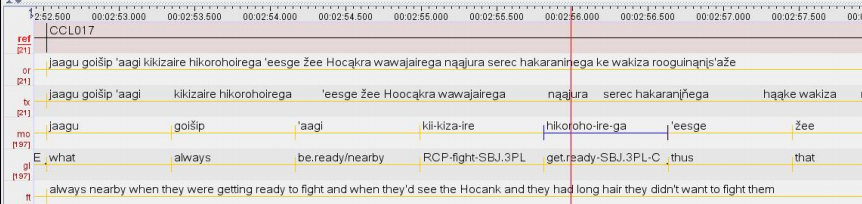
\includegraphics[width=0.75\columnwidth]{ELAN.png}
\caption{Interlinearization in ELAN.}
\end{center}
\end{figure}

Popular linguistic software tools that aid interlinearization do not incorporate computational morphological models. So, unfortunately, NLP help is not available to linguists who do not have computer programming skills. ELAN, shown in Figure \ref{fig:ELAN}\footnote{Source: \newcite{bouda_corpus_2012}}, and FLEx, shown in Figure \ref{fig:FLEX}\footnote{Source: http://software.sil.org/fieldworks/resources/tutorial/interlinearize-texts/} are two popular tools. Neither use machine learning to aid segmentation or glossing, although they do present suggestions, but only if a word form is identical to one that was previously annotated. Instead, linguistic annotation is performed primarily by hand, and while human analysis is the most reliable because a human is much better able to interpret contextual cues, once the initial analysis is complete, manual annotation is extremely inefficient \cite{Baldridge06,baldridge_how_2009,palmer_semi-automated_2009}. Interlinearization is repetitive and monotonous, and, therefore, prone to typos and inconsistencies when done manually. Manual annotation is costly, requiring money and time to hire and train annotators. It is time-consuming; even in computational linguistics it took three years to annotate just one layer of the Penn Treebank \cite{taylor_penn_2003} \cite{duong_natural_2017,he_humanloop_2016}. A documentary field project may record several hours of valuable and endangered data, but interlinearization is rarely completed within funding and time limits. This situation persists, even though it has been known for some time that machine learning can be effectively applied to the LDD data annotation \cite{baldridge_how_2009,palmer_semi-automated_2009,duong_natural_2017}.

\begin{figure}[ht]
\begin{center}
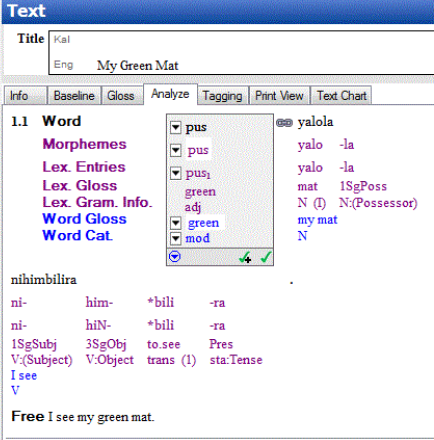
\includegraphics[width=0.40\columnwidth]{FLExIGT.png}
\caption{Interlinearization in Fieldworks Language Explorer (FLEx).}
\label{fig:FLEX}
\end{center}
\end{figure}

\subsection{What can be done now}
\label{sec:splicing}
The bottleneck of interlinearization can be addressed right now using existing computational approaches. With some manual pre-annotation, supervised learning models can speed interlinearization and support fuller morphological description. By simply splicing together some of the approaches described in this paper, it is likely that the time costs can be reduced by 80-90\% \cite{moeller_automatic_2018}. There are many ways to do this. This subsection outlines just one possibility.

To address segmentation and glossing, a CRF with simple, cross-linguistic features can be trained on previously segmented data. Such a model has achieved over 93\% accuracy using only 3,000 training words to segment and label the closed class of affixes in Lezgi \cite{moeller_automatic_2018}. (see section \ref{sec:supervised} On the open class of roots, accuracy will be lower, but can be improved with some techniques described in section \ref{resources}. For example, existing dictionaries or lexicons or an FST can be exploited to increase training data for a neural model \newcite{moeller_neural_2018} and \newcite{moeller_improving_2019} (see section \ref{sec:NN}.) If these resources are insufficient, then word lists from languages with heavy borrowings can be used as \newcite{baumann_using_2014} did (see section \ref{transfer}). Replicating and testing these approaches on documentary data in other languges will indicate which one works best with a given morphological type or language family. If necessary, new techniques can be explored. For example, a neural morphological analysis model can be augmented during training by adding the words surrounding the target word in the text; or a joint model can be trained with POS tag if the LDD project included them.

The  approaches described in this paper, particularly in section \ref{paradigms} regarding paradigm induction, can not only speed and improve interlinearization but can also serve as a jumpstart for identifying inflectional classes and their paradigms. For example, once a significant amount of texts have been morphologically segmented and glossed, the approach used by \newcite{ahlberg_paradigm_2015} and illustrated in Figure \ref{fig:LCS} (see section \ref{paradigms}) can be applied to suggest candidate inflectional patterns. With slight adjustment it can output the lexemes identified with each pattern and group them into candidate inflectional classes. These candidate paradigm tables and inflectional class identification can serve as working hypotheses for the linguist who is broadening the morphological description of a language.

\textbf{Other Low-Hanging Fruit.} The plan outlined above only uses approaches described in this paper but it does not address all three parts of interlinearization.  To complete free translation, the third line of interlinearized texts\footnote{Also known as interlinearized glossed texts or IGTs}, a machine translation model can be added to the workflow once a significant amount of text has been morphologically glossed. An encoder-decoder translation model can learn to ``translate'' the glossed lines into ``bad English'', then ``translate'' that into ``good'' English (or Spanish or Russian or whatever high resource language is desired). The progression looks like that in example \ref{ex:MT} which begins with the gloss of a Russian sentence.

\begin{singlespace}
\pex<transl> 
\label{ex:MT}
evening\textsc{-inst} \textsc{1sg} run\textsc{-past.sg.fem} in store\textsc{-acc} $\longrightarrow$ \\
`Evening with I ran in store to' $\longrightarrow$ \\
`In the evening I ran to the store.'
\xe
\end{singlespace}

It would be wonderful to begin machine-aided morphological analysis as soon as transcribed data becomes available, but automated support can be more time-consuming than manual annotation if the model performs poorly \cite{kothur_document-level_2018,palmer_semi-automated_2009}. Introducing existing machine learning models at specific points in the LDD workflow as described above assumes that annotators pre-annotate a portion of a corpus. A key question then is how much data should a LDD project annotate before training the computational model? This question would be difficult to answer as it might depend on the morphological type or the type of annotation. The next section bysteps this by going beyond the approaches discussed in this paper by including active learning which can quickly improve a model even with a small amount of supervised data. 

\subsection{What should be done in the near future}

The plan in the previous subsection is mostly limited to the techniques and models described in this paper, but adding one more machine learning technique, computational linguistics could contribute considerably more to the interlinearizing annotation process (and receive increased training data in return). \newcite{baldridge_how_2009} propose two stratagems to improve and speed annotation: reduce the cost of annotating new data or get more miles out of previously annotated data. Crowdsourcing is an example of the first strategem but has proved less effective in low resource contexts \cite{bird_aikuma:_2014,bettinson_developing_2017}. For the second strategem, Baldridge et al. recommend active learning, which is a machine learning technique ideal for situations where raw data is abundant but manual annotation is expensive. 

Active learning is conducted in an iterative cycle of annotating data and training a supervised model. After the model is trained and tested, it is run on unseen data. Human annotators are then directed towards a certain number of the most informative samples in that data. Informative samples are those most likely to improve the model upon re-training (e.g. word forms most dissimilar to any in the training data). Annotators manually vet and correct the model's predictions for these samples.\footnote{This step is done manually, but \newcite{rocio_detection_2007} found that even this can be semi-automated if the model's patterns of errors are identified.} With these corrected annotations included the model is re-trained. The cycle continues until desired accuracy is achieved or the point of diminishing returns from re-training is reached. The last bit of raw data is vetted and corrected by hand.

Experiments in computer-aided machine translation \cite{kothur_document-level_2018} and interlinearizion \cite{palmer_semi-automated_2009,palmer_evaluating_2009,palmer_computational_2010} indicate that active learning is a very promising route for LDD tasks. Active learning applied with computational morphological models to an Uspanteko [usp] documentary corpus gave a significant boost in the models' accuracy \cite{palmer_semi-automated_2009}. At the same time, the annotators' productivity was increased and the time cost of annotation greatly reduced.

\begin{figure}[ht]
\label{fig:ML-LDD}
\begin{center}
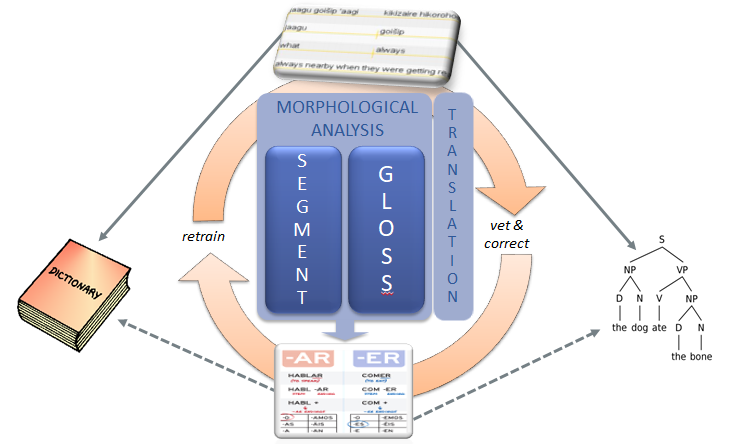
\includegraphics[width=0.75\columnwidth]{ML-LDD.PNG}
\caption{A practical application of computational morphology to language documentation and description would focus on addressing the time costs of interlinearizing transcribed texts (1). Incorporating computational morphological models at the segmentation and glossing steps (2) could feed into machine translation models (3) that would help complete the interlinearization and then into paradigm induction models which could provide working hypotheses of inflectional patterns and classes (4). This would support the development of dictionaries (5) and full grammatical descriptions (6). Even with very limited initial supervised the models can continue to improve if a cycle of active learning (7) is introduced at one or multiple points in this workflow. This allows annotators to vet and correct the most informative of the models' prediction and then use that information to efficiently retrain the models.}
\end{center}
\end{figure}

The iterative nature of active learning calls for human interaction. Unfortunately, ``ordinary working linguists'' and the average native speaker annotator would not find the typical model's output easy to work with, and may actually find them intimidating. If computational linguistics wishes to benefit general linguistics and receive benefit from its increased productivity, this gap of skills and knowledge must be bridged. Therefore, the development of well-designed graphical user interfaces is vital. A good interface would be attractive and easy-to-navigate, drawing from user experience expertise and user feedback. An interface for active learning would not only walk annotators through the steps of annotating data and training a model, but its graphics would draw their attention to samples that most need to be vetted or corrected and recommend when re-training should take place. The value of such an interface can be seen by contrasting the interface provided by ELPIS \cite{foley_elpis_2018}, a wonderful application of machine learning to the LDD transcription bottleneck. It does not indicate any kind of confidence score where the model likely to have transcribed an incorrect symbol. Instead, it leaves the annotator to examine each and every symbol to find and correct errors. 

A good interface for active learning could be reused for many tasks such as transcription and POS-tagging, as well morphological segmentation and glossing. It might mean new features or else an add-on in existing software such as ELAN \cite{auer_elan_2010} and FLEx \cite{Black06FLEX}. It might mean a new software program that is compatible with popular tools, as for example, ELPIS which is a web-based app that intakes and outputs data in ELAN-compatible format.  

Ideally, linguists will someday spend minimal time on manual interlinearization and other linguistic annotation, followed by a few cycles of training a supervised machine learning model, vetting and correcting its results, and retraining the model until it achieves extremely high accuracy. The primary question is not whether a LDD project annotated sufficient data, but how many rounds of re-training and manual correction will be required before it becomes more expensive than finishing the annotation by hand. 

\section{Conclusion}
All computational morphological models—finite state transducers, unsupervised, supervised feature-based or neural networks, and semi-supervised---need data. Unsupervised models achieve some success with unannotated data, but accuracy is much higher with supervised and semi-supervised machine learning which require annotated data. Despite the importance of annotated data, the computational linguistics literature repeatedly returns to the unfortunate reality that ``annotating sufficient data...is expensive'' \cite[page 1954]{cotterell_cross-lingual_2017}. This has retarded the development of NLP and its potential contribution to linguistic science. The literature adds another perceived inconvenience: that annotation ``relies on linguistic expertise'' (\textit{ibid}). That is, a language expert—native speaker or linguist—must be involved to produce gold standard annotations necessary for training and evaluating machine learning models or for building finite state machines.

Morphological annotation of texts (interlinearization) also stands as a bottleneck to language documentation and language description \cite{bird_documentary_2015,bettinson_developing_2017,holton_developing_2017}. It is not, however, the ``inconvenient'' reliance on people who actually know the language. Making the most of native speaker knowledge has long been an integral part of linguistics and language documentation literature is brimming with proven methods for doing so. What is remains is the need to reduce the cost of annotation and speed its production even while existing resources are few. 

Fortunately, computational approaches are being increasingly applied to low resource contexts and are achieving reasonable success. This paper compared various computational approaches to morphological analysis. It described much of what has already been accomplished in low resource contexts. Finally, it presented how this trend has the potential to address practical needs and bottlenecks in the language documentation and language description workflow. It outlined a plan to incorporate existing models and then suggested that active learning and well-designed user interfaces are the strategic next steps to speed and improve the production of annotated data. 

Bridging this technological gap between computational morphology and language documentation and description will undoubtedly open new questions for future research. For NLP, the questions are likely to focus on how models and techniques should adjust so that they perform optimally across a wide range of languages. For linguistics, a big question is likely to how machine learning will affect best practices in field methods. Future work must seek an optimal balance between NLP goals and the priorities of field linguists, as well as the priorities and needs of the communities who speak low resource, and often endangered, languages. 

\newpage

\bibliographystyle{acl}
\bibliography{0_References}
\end{document}
